\chapter{Ejercicio Sigue Personas simulado en Robotics Academy}
\label{cap:capitulo5}

En este capítulo se presenta la elaboración del ejercicio Follow Person para Robotics Academy empezando desde el desarrollo interno de la infraestructura del ejercicio hasta una solución óptima de referencia que realice la tarea de seguir a una persona.



% -- SECCION ENTORNO GAZEBO
% ---------------------------
\section{Entorno simulado de un hospital}
\label{sec:hospital_gazebo}

La primera tarea fue integrar un entorno para Gazebo en el cual el robot Turtlebot2 tendría que enfrentarse. El entorno candidato que elegimos fue un \textbf{Hospital} debido a las siguientes ventajas:

\begin{enumerate}
	\item El robot se enfrenta a un entorno complejo (paredes, obstáculos, varias personas).
	\item La tarea Sigue Personas tendría lugar en un entorno en el cuál tiene sentido verlo en el mundo real. Los Robots en el ámbito de la salud están en continua integración.
\end{enumerate}

De modo que incorporamos el siguiente mundo de Gazebo que proporciona AWS (Amazon Web Service) en uno de sus repositorios de Github \footnote{\url{https://github.com/aws-robotics/aws-robomaker-hospital-world}}:

\begin{figure} [H]
  \begin{center}
    \includegraphics[width=10cm]{imagenes/hospital_world.png}
  \end{center}
  \caption[Hospital de AWS en Gazebo]{Hospital de AWS en Gazebo}
  \label{fig:hospital_gazebo}
\end{figure}

El repositorio proporcionaba varios ficheros \textbf{.world} con distintas versiones del Hospital: solo planta baja, una planta y dos plantas. Elegimos por comodidad la primera.\\

El siguiente paso era integrar una persona que pudiera desplazarse por el entorno.



% -- SECCION TELEOPERADOR
% -------------------------
\section{Teleoperador}
\label{sec:teleoperador}

El objetivo final es que el usuario que use la plantilla web pueda mover manualmente una persona del Hospital para que el robot pueda seguirla. Para ello teníamos que desarrollar un teleoperador.\\

El primer punto de partida era integrar una persona en el nuevo entorno simulado, por lo que accedimos a este repositorio \footnote{\url{https://github.com/osrf/gazebo_models}} que incorpora una librería de modelos para Gazebo e insertamos en el repositorio de Robotics Academy de terceros \textbf{Custom Robots} el modelo \textbf{\textit{person standing}}

\begin{figure} [H]
  \begin{center}
    \includegraphics[width=10cm]{imagenes/person_model.png}
  \end{center}
  \caption[Persona simulada en Gazebo]{Persona simulada en Gazebo}
  \label{fig:persona_gazebo}
\end{figure}

Ahora bien, el modelo es estático, carece de capacidad de desplazamiento, por lo que fue necesario desarrollar un plugin para Gazebo que permitiera ser controlado o que pueda desplazarse a través de una ruta que eligiera el programador. De modo que en el mismo paquete donde tenía los ficheros de lanzamiento del hospital diseñe el plugin (escrito en C++) al que denominé \textbf{libpersonplugin.so} para incorporarlo en el fichero \textbf{.sdf} (similar a URDF) de la persona. En este enlace podréis ver el \textbf{código fuente}\footnote{\url{https://github.com/JdeRobot/CustomRobots/blob/foxy-devel/amazon_hospital/hospital_world/src/person.cpp}}\\

El plugin requiere \textbf{2 funcionalidades}:
\begin{enumerate}
	\item \textbf{Comunicación remota} para el control manual. La intención es que el usuario se comunique con el modelo simulado, por lo tanto diseñé un \textbf{socket} de comunicaciones para dicha tarea.
	\item \textbf{Establecimiento de una ruta} por defecto y capacidad de incorporar nuevas rutas. Esta última funcionalidad no es necesaria para el ejercicio, además de que puede suponer cierta molestia al usuario, pero no se descarta su utilidad para un futuro.
\end{enumerate}

% -- SUBSECCION COMUNICACION REMOTA
% ----------------------------------
\subsection{Comunicación remota}
\label{subsec:comunicacion_remota}

En el propio fichero \textbf{person.cpp} creé 2 hilos (threads). Uno actuaría como servidor de un socket de comunicaciones que usaría el protocolo de transporte \textbf{UDP} (No esta orientado a la conexión y es más rápido). Dentro del socket implementé un protocolo de comunicación que entendierá el servidor, el cual sería únicamente receptor de los mensajes del cliente. Los mensajes que puede recibir son:

\begin{itemize}
	\item \textbf{``UVF"} (User Velocity Forward). El modelo se mueve hacia delante.
	\item \textbf{``UVB"} (User Velocity Backward). El modelo se mueva hacia atrás.
	\item \textbf{``UAR"} (User Angular Right). El modelo gira hacia la derecha.
	\item \textbf{``UAL"} (User Angular Left). El modelo gira hacia la izquiera.
	\item \textbf{``US-"} (User Stop). El modelo se detiene.
	\item \textbf{``A--"} (Autonomous). El modelo pasa a modo autónomo. Sigue la ruta establecida (actualmente desactivada).
\end{itemize}

Pero ¿dónde entra en juego el cliente? El fichero \textbf{exercise.py} incorpora un socket de comunicación UDP que se conecta al servidor del plugin a través del puerto 36677. Además, el \textbf{exercise.py} es el servidor de un WebSocket en comunicación con la plantilla web. Cuando el usuario haga click en el botón ``Teleoperate", el fichero de eventos de Javascript podrá enviar a través de un Websocket, que usa el puerto 1905, las teclas pulsadas para que el exercise.py se lo retransmita al plugin. Al iguál que en la comunicación \textbf{plugin-exercise.py}, implementé un protocolo de comunicación para \textbf{exercise.py-exercise.html}. Los mensajes que puede recibir son:

\begin{itemize}
	\item \textbf{``\#teleop\_true"}. Activa la teleoperación. A partir de ese momento, el usuario puede pulsar los botones ``awsdx". Envía un mensaje \textbf{``US-"} al plugin.
	\item \textbf{``\#teleop\_false"}. Desactiva la teleoperación. Pasa a modo autónomo (si estuviera activado). Envía una mensaje \textbf{``A--"} al plugin.
	\item \textbf{``\#key\_a"}. Envía un mensaje \textbf{``UAR"} al plugin.
	\item \textbf{``\#key\_d"}. Envía un mensaje \textbf{``UAL"} al plugin.
	\item \textbf{``\#key\_w"}. Envía un mensaje \textbf{``UVF"} al plugin.
	\item \textbf{``\#key\_s"}. Envía un mensaje \textbf{``UVB"} al plugin.
	\item \textbf{``\#key\_x"}. Envía un mensaje \textbf{``US-"} al plugin.
\end{itemize}

A continuación podemos ver un esquema que resuma la comunicación existente entre el exercise.html (incorpora el fichero ws\_code.js) con el plugin:

\begin{figure} [H]
  \begin{center}
    \includegraphics[width=15cm]{imagenes/comunicacion-teleoperador.png}
  \end{center}
  \caption[Comunicación del teleoperador]{Comunicación del teleoperador}
  \label{fig:comunicacion_teleoperador}
\end{figure}

% -- SUBSECCION DESPLAZAMIENTO DEL MODELO
% -----------------------------------------
\subsection{Desplazamiento del modelo}
\label{subsec:desplazamiento_modelo}
(TODO)




% -- SECCION HAL
% ----------------
\section{Desarrollo de la Capa de Abstracción Hardware (HAL)}
\label{sec:turtlebot2_hal_simulado}

\begin{figure} [H]
  \begin{center}
    \includegraphics[width=15cm]{imagenes/vista-planta-turtlebot2.png}
  \end{center}
  \caption[Láser Turtlebot 2]{Láser Turtlebot 2}
  \label{fig:vista_planta_turtlebot2}
\end{figure}
(TODO)




% -- SECCION SIGUE PERSONAS
\section{Solución Sigue-Personas Simulado}
\label{sec:sigue_personas_simulado}

En esta sección explicaremos la elaboración de una solución de referencia para el problema Sigue Personas de este ejercicio en simulado. La solución la podemos dividir en 3 subobjetivos: a) detección mediante Machine Learning y seguimiento mediante un Tracker, b) desarrollo de un algoritmo de evitación de obstáculos y c) creación de una máquina de estados.

\subsection{detección mediante ML y creación de un Tracker}
\label{sec:ml_tracker}
Para detectar a la persona usaremos la función del módulo HAL llamada \textbf{getBoundingBoxes}. Esta función realiza una ejecución sobre el modelo de red neuronal para detectar todos los objetos posibles dada una \textbf{imagen} de entrada y devuelve una lista de objetos \textbf{Bounding Box} (TODO explicados en la sección anterior). Crearemos una función llamada \textbf{\textit{draw\_bounding\_box(img, bbox, color=(23, 230, 210), thickness=2)}} con la que podremos dibujar sobre la imagen un Bounding Box dado como entrada. En este caso usaremos el color verde (0, 255, 0) e iteraremos sobre todos los Bounding Boxes obtenidos (Figura \ref{fig:deteccion_ssd_sin_filtro})\\

\begin{figure} [H]
  \begin{center}
    \includegraphics[width=10cm]{imagenes/deteccion-ssd-sin-filtro.png}
  \end{center}
  \caption[Detección mediante SSD sin filtro]{Detección mediante SSD sin filtro}
  \label{fig:deteccion_ssd_sin_filtro}
\end{figure}

Sin embargo, un modelo de red neuronal genera una \textbf{puntuación} o \textbf{score} para cada objeto detectado dependiendo de su entrenamiento, por ejemplo, en una imágen donde puede aparecer una persona y una escultura humana, es probable, que la persona detectada tenga una puntuación de un 90 \% y la escultura un 70 \% debido a su parecido. Está en la labor del programador filtrar por score para desechar los \textbf{falsos positivos}. Para ello, generamos una función que llamaremos \textbf{\textit{bounding\_boxes\_by\_score(bounding\_boxes, score\_limit)}} que filtre aquellos bounding boxes que superen una puntuación límite. Debido a la naturaleza de este modelo neuronal preentrenado, las óptimas detecciones se han comprobado empíricamente que funcionan con una puntuación superior a \textbf{0.3} (el rango es de 0 a 1). Aplicando el filtro obtenemos el siguiente resultado (Figura \ref{fig:deteccion_ssd_filtro_score})\\

\begin{figure} [H]
  \begin{center}
    \includegraphics[width=10cm]{imagenes/deteccion-ssd-filtro-score.png}
  \end{center}
  \caption[Detección mediante SSD filtrando el \textbf{Score}]{Detección mediante SSD filtrando el \textbf{Score}}
  \label{fig:deteccion_ssd_filtro_score}
\end{figure}

Tal y como vemos en la figura \ref{fig:deteccion_ssd_filtro_score}, tras el filtro de \textbf{puntuación} obtenemos una imagen donde hay 3 Bounding Boxes detectados: una persona y 2 sillas. Para quedarnos solo con las personas aplicaremos un \textbf{segundo filtro}, en la cual nos fijaremos en la \textbf{clase} del Bounding Box. Recordemos que el objeto Bounding Box tenía un atributo \textbf{id} que correspondía a un número entero y un atributo \textbf{class\_id} que era la traducción de dicho número a una cadena de texto (ej: 1 - ``person", 2 - ``bicycle"). Crearemos una función llamada \textbf{\textit{bounding\_boxes\_by\_name(bounding\_boxes, name)}} al cual dada una lista de objetos detectados pasaremos como segundo parámetro de entrada el nombre de la clase que queremos filtrar (en este caso ``person"). Aplicando el filtro obtenemos una correcta detección de personas (Figura \ref{fig:deteccion_ssd_filtro_score_class}):

\begin{figure} [H]
  \begin{center}
    \includegraphics[width=10cm]{imagenes/deteccion-ssd-filtro-score-class.png}
  \end{center}
  \caption[Detección mediante SSD filtrando el \textbf{Score} y la \textbf{Clase}]{Detección mediante SSD filtrando el \textbf{Score} y la \textbf{Clase}}
  \label{fig:deteccion_ssd_filtro_score_class}
\end{figure}

Como último filtro y muy recomendable es rechazar aquellas detecciones que no superen un \textbf{área} determinado. Con este filtro, evitamos que el robot se confunda con personas que se encuentren a una distancia lejana o con un falso positivo, para ello, crearemos una función llamada \textbf{\textit{bounding\_boxes\_by\_area(bounding\_boxes, min\_area)}} al cual dada una lista de objetos detectados pasaremos como segundo parámetro de entrada el área mínima que debe filtrar.\\

El siguiente paso es crear un \textbf{Tracker} de seguimiento. Nuestro tracker se basará en la distancia de los centroides de los Bounding Boxes de un fotograma el candidato anterior. Recordemos que un Bounding Box tenía otros 4 parámetros más: xmin e ymin correspondían a las coordenadas (x,y) del extremo superior izquierdo de la caja de detección, y xmax e ymax correspondían a las coordenadas (x,y) del extremo inferior derecho. Para obtener el \textbf{centroide} aplicaremos la siguiente fórmula:\\
\begin{eqnarray*}
C_x = \frac{x_{min} + x_{max}}{2}\\
C_y = \frac{y_{min} + y_{max}}{2}\\
\end{eqnarray*}

Crearemos una clase llamada \textbf{BoundingBoxObject} que tendrá 3 atributos: El \textbf{Bounding Box} correspondiente, su \textbf{centroide} y el \textbf{área}. El área lo calcularemos tal que así: $A = (x_{max} - x_{min}) (y_{max} - y_{min})$\\

Posteriormente, creamos una clase llamada \textbf{Tracker} que nos proporcionará una capa de abstracción al usar los siguientes métodos que definiremos:
\begin{itemize}
	\item \textbf{\textit{setObjective(self, obj)}}: Establece el objetivo BoundingBoxObject de seguimiento.
	\item \textbf{\textit{getObjective(self)}}: Devuelve el objetivo BoundingBoxObject actual de seguimiento.
	\item \textbf{\textit{getObjectiveFromSet(self, objlist)}}: Dada una lista o conjunto de objetos BoundingBoxObject, devuelve el objetivo candidato que más se acerca al anterior, y lo actualiza. El candidato seleccionado será aquel cuyo centroide esté más cerca al actual, que no supere una distancia límite de diferencia(50) y que la diferencia de área entre el BoundingBoxObject anterior y el actual sea menor a 30000. Para calcular la distancia entre centroides usaremos la Distancia Euclídea:
	\begin{equation*}
	d = \sqrt{(C_{x}' - C_{x})^2 + (C_{y}' - C_{y})^2}
	\end{equation*}
\end{itemize}

En la figura \ref{fig:obtencion_centroide} podemos ver con más detalle en que se basa esté procedimiento: comparamos cada centroide con el centroide candidato del fotograma anterior y elegiremos aquel que cumpla los requisitos descritos anteriormente.
\begin{figure} [H]
  \begin{center}
    \includegraphics[width=10cm]{imagenes/esquema-tracker.png}
  \end{center}
  \caption[Modo de obtención del centroide candidato]{Modo de obtención del centroide candidato}
  \label{fig:obtencion_centroide}
\end{figure}

En cada iteración del bucle principal del programa cuando llamemos al método \textbf{getObjectiveFromSet()} de la clase Tracker obtendremos un BoundingBoxObject el cual dibujaremos en la imagen de color rojo. El resultado sería el siguiente:


 

